\documentclass{amsart}
\usepackage{amsfonts, amsthm, amssymb, amsmath}
\usepackage{mathtools}
\usepackage{graphicx,caption,subcaption}
\usepackage{comment}
\usepackage{xcolor}
\usepackage{tikz}
%\usetikzlibrary{decorations.markings,arrows.meta,calc,fit,quotes,cd,math,external}
\usetikzlibrary{
  matrix,
  arrows,
  arrows.meta,
  calc,
  fit,
  quotes,
  cd,
  math,
  external,
  shapes,
  decorations.markings,
  decorations.pathreplacing,
  patterns,
  decorations.pathmorphing
}

\usepackage{url}
\usepackage[inline]{enumitem}
	\setlist{itemsep=0em, topsep=0em, parsep=0em}
	\setlist[enumerate]{label=(\alph*)}
\usepackage[all,2cell]{xy}\UseAllTwocells\SilentMatrices
\usepackage[breaklinks=true]{hyperref}%John's choices, can change; previous choice \definecolor{hyperrefcolor}{rgb}{0,0,0.7}
\definecolor{darkgreen}{rgb}{0,0.45,0}
\definecolor{myurlcolor}{rgb}{0.6,0,0}
\definecolor{mycitecolor}{rgb}{0,0,0.8}
\definecolor{myrefcolor}{rgb}{0,0,0.8}
\hypersetup{colorlinks, linkcolor=myrefcolor, citecolor=darkgreen, urlcolor=myurlcolor,
final,linktoc=page}
\usepackage[capitalize]{cleveref}
\crefname{equation}{}{}
\crefname{item}{}{}
\crefname{prop}{Proposition}{Propositions}

%
% environments and counters
%

\newtheorem{thm}{Theorem}[section]
\newtheorem{cnj}[thm]{Conjecture}
\newtheorem{lem}[thm]{Lemma}
\newtheorem{prop}[thm]{Proposition}
\newtheorem{cor}[thm]{Corollary}

\theoremstyle{remark}
	\newtheorem{remark}[thm]{Remark}
	\newtheorem{notation}[thm]{Notation}

\theoremstyle{definition}
	\newtheorem{ex}[thm]{Example} 
	\newtheorem{defn}[thm]{Definition}

% math text formatting
\newcommand{\cat}[1]{\mathsf{#1}}

% common category names

\newcommand{\Set}{\cat{Set}}
\newcommand{\Grph}{\cat{Grph}}
\newcommand{\Cat}{\cat{Cat}}
\newcommand{\twoCat}{\cat{2Cat}}
\newcommand{\Adj}{\cat{Adj}}
\newcommand{\one}{\mathbf{1}}
\newcommand{\two}{\mathbf{2}}
\newcommand{\Fib}{\cat{Fib}}
\newcommand{\OpFib}{\cat{OpFib}}
\newcommand{\Corefl}{\cat{Corefl}}
\newcommand{\Rali}{\cat{Rali}}

\newcommand{\C}{\cat{A}}
\newcommand{\D}{\cat{X}}
\newcommand{\A}{\cat{A}}
\newcommand{\X}{\cat{X}}
\newcommand{\U}{U}
\newcommand{\Q}{Q}
\renewcommand{\L}{L}
\newcommand{\R}{R}
\renewcommand{\P}{P}
\newcommand{\B}{\cat{B}}
\newcommand{\Y}{\cat{Y}}

\newcommand{\Cocart}{\mathrm{Cocart}}
\newcommand{\Cart}{\mathrm{Cart}}

\newcommand{\op}[1]{\operatorname{#1}}
\renewcommand{\t}[1]{\text{#1}}

\newcommand{\from}{\colon}
\newcommand{\xto}[1]{\xrightarrow{#1}}
\newcommand{\To}{\Rightarrow}
\newcommand{\Tto}{\Rrightarrow}
\newcommand{\bydef}{\coloneqq}
\newcommand{\define}{\textbf}%consider change to bold? or something else?

%
% math operators
%

\DeclareMathOperator{\Hom}{Hom}
\DeclareMathOperator{\id}{id}
\DeclareMathOperator{\ob}{Ob}
\DeclareMathOperator{\arr}{arr}
\DeclareMathOperator{\im}{im}
\DeclareMathOperator{\Aut}{Aut}
\DeclareMathOperator{\Bij}{Bij}
\DeclareMathOperator{\Sub}{Sub}
\DeclareMathOperator{\colim}{colim}
\newcommand{\iso}{\cong}

%
% tikz styles
%

% arrows for commuting diagram
\tikzset{
  cd/.style={
    ->,
    scale=6,
    >=angle 90,
    font=\scriptsize}
  }

% its us!

\definecolor{purple(x11)}{rgb}{0.5, 0.0, 0.5}
\newcommand{\chris}{\color{purple(x11)}}
\newcommand{\daniel}{\color{red}}


\newcommand{\nice}{\emph{nice}}

\begin{document}
\title{Fibrations and Adjunctions}

\author{Daniel Cicala and Christina Vasilakopoulou} 
\address{Departement of Mathematics, University of California, Riverside, 900 University Avenue, 92521, USA}
\email{cicala@math.ucr.edu,vasilak@ucr.edu}

\begin{abstract}
Fibrations and Adjunctions rock.
\end{abstract}

\maketitle

\tableofcontents

\section{Introduction}
{\chris Christina's questions to Steve:}

I had a question regarding choice of (co)limits in categories. Please excuse my naivety, I haven't really gone into depths of such
questions before because I guess if one can avoid them, they tend to! But any insight or 'big picture' idea from you would be really,
really appreciated to help me understand better a situation I find myself in. In particular, feel free to correct me in the following
statements.

(1) 'Choosing limits' in a complete category amounts to choosing a specific (of the many isomorphic ones) adjoint to the
constant diagram functor. Therefore if a category has limits, we can assume it has chosen ones. Does this already require the axiom of
choice?

(2) Therefore this choice is already 'functorial'. However, can we 'choose the choice'? In particular, is it reasonable
to say that if C has pushouts for example, there is such a specific choice such that the pushout of f along the identity 'is'
exactly f (and the identity)?

(3) If a functor $F:C\to D$ between categories with pushouts preserves them in the ordinary sense, can we actually make a
choice of them in C and in D, such that F strictly preserves them? What assumptions should I make to be able to do that?
Or this is somehow extra, i.e. needs to be checked or required?

Thanks so much in advance for any intuition that would help wrap my head around these!

A quick question to end: it is a fact that every Grothendieck fibration is a particular case of Street fibration,
and I also read that every Street fibration factors as an equivalence of categories followed by a Grothendieck one.
(I am in the process of reading Street's paper, but) does this by any chance induce an equivalence of categories? Fib with StreetFib?

{\chris Steve's response:}

1. As you say, choosing limits amounts to choosing a specific adjoint to the diagonal functor (with corresponding
statements holding if you are using weighted limits). I certainly allow myself to regard a category with limits as having
chosen ones if I wish. I suppose from a formal point of view that does require the axiom of choice, but I also use this as necessary.
The category of sets does have a canonical choice, which means that many of the most commonly occurring complete categories
also have a canonical choice.

2. Functoriality is automatic, irrespective of choice issues. There is also no problem with first using the canonical
choice where it exists (for example with pushouts along identities) and then extending this arbitrarily to deal with other cases.
I guess that once again you need the axiom of choice for this, but are you actually worried about that?

3. I have never thought about this - at first sight it seems a bit unnatural. In any case, I think that this
is not automatic. Let $2={0->1}$ be the arrrow category, and let $C=2\times 2\times 2$ be the free-living commutative cube.
Each face of the cube is in fact a pushout; in fact C has a unique choice of pushouts. Let D be the category obtained from the
square $2\times 2$ by adding an extra object c isomorphic to (1,1). Then D contains two commutative squares:
the original 2x2, and one using the new object. This category once again has pushouts, but now there are choices to make.
There is an evident (unique) functor f:C->D sending the top face of the cube to the first square and the bottom
face the second square. Whatever choice of pushouts you make in D, either the pushout in the top face of
C or that in the bottom face will fail to be preserved strictly.

Regarding your question about fibrations, there is a question as to what your �categories of fibrations� are.
But perhaps more natural would be to consider 2-categories, and then look for a biequivalence between these. This can be done.



\section{Preliminaries}

Mainly basics of fibrations and adjunctions, to fix terminology. Also Street stuff.

\section{Sth}
Gray's and our theorem as one big thing. Maybe start from Street, and restrict to Grothendieck.

Then, monoidal analogue.

Then, probably lift to (2-)categories of such things.


[Here probably ends more or less what is needed for network big picture. Surely we can think of other things we wanna say.]

%We are closing in on a pair of theorems.

%\begin{thm}
%	Fix an adjunction 
%	\[
%	\begin{tikzpicture}
%		\node (C) at (0,0) {$ C $}	;
%		\node (D) at (2,0) {$ D $}	;
%		\draw [->] (C.30) to node {$ L $} (D.150);
%		\draw [->] (D.210) to node [swap] {$ R $} (C.-30);
%	\end{tikzpicture}
%	\]
%	$ R $ is a Street opfibration if and only if the adjunction in \nice.	
%\end{thm}


%\begin{equation}\label{factor}
%\xymatrix @C=.4in @R=.2in
%{A\ar[rr]^\theta\ar @{-->}[d]_-{\psi} && B \ar @{.>}[dd] &\\
%f^*B\ar[urr]_-{\;\Cart(f,B)} \ar @{.>}[d] &&& \textrm{in }\ca{A} \\
%X\ar[rr]_-{f} && Y & \textrm{in }\caa{X},}\qquad
%\xymatrix @C=.4in @R=.2in
%{C \ar @{.>}[dd]\ar[rr]^\gamma \ar[drr]_-{\Cocart(g,C)} && D &\\
%&& f_!C \ar @{-->}[u]_-{\delta} \ar @{.>}[d] & \textrm{in }\ca{C} \\
%X\ar[rr]_-{g} && Y & \textrm{in }\caa{X}.}
%\end{equation}

\subsection{Newer}

Recall that \emph{lari} is an acronym for `left adjoint, right inverse', the latter meaning that the unit of %be careful, TRICKY! for rari, it is the counit!
the adjunction is the identity. For example, if $G\colon\cat{D}\to\cat{C}$ has a lari $L$, then $L\dashv G$ and
$\eta\colon1_\cat{C}=GL$. Notice that if a functor has a \emph{rari} analogously, then the counit is the identity instead.
 The following result is the dual of \cite[Prop. 4.4]{Grayfibredandcofibred}.

\begin{prop}
 Let $U\colon\cat{D}\to\caa{C}$ be an opfibration. Then its fibres have initial objects which are preserved by the reindexing functors
 if and only if $U$ has a lari.
\end{prop}

\begin{proof}
Denote by $\bot_x$ the initial object in each fiber $\cat{D}_x$ above an object $x\in\caa{C}$. Define the left adjoint
of $U$ as follows:
\begin{displaymath}
\begin{tikzcd}[row sep=.1in]
L\colon\caa{C}\ar[rr] && \cat{D} &\\
x\ar[rr,mapsto]\ar[dd,"f"'] && \bot_x\ar[dd,dashed,"Lf"']\ar[ddr,"{\Cocart(f,\bot_x)}"] & \\
\hole \\
y\ar[rr,mapsto] && \bot_y\ar[r,"\cong"] & f_!(\bot_x)
\end{tikzcd}
\end{displaymath}
This mapping is well-defined and functorial due to the universal properties of cocartesian liftings.
To show it is a left adjoint of $U$, it suffices to establish a natural bijection
$\cat{D}(Lx,a)\cong\caa{C}(x,Ua)$ for any $x\in\caa{C}$, $a\in\cat{D}$. Indeed, each morphism
$k\colon Lx\to a$ above $f=Uk$ factorizes uniquely as
\begin{displaymath}
\xymatrix @C=.5in @R=.3in
{\bot_x \ar @{.>}[dd]\ar[rr]^k \ar[drr]_-{\Cocart(f,\bot_x)} && a &\\
&& f_!(\bot_x) \ar @{-->}[u]_-s \ar @{.>}[d] & \textrm{in }\cat{D} \\
x\ar[rr]_-{f} && Ua & \textrm{in }\caa{C}}
\end{displaymath}
but since $f_!(\bot_x)\cong\bot_{Ua}$ is the initial object, the morphism $s$ is unique
and thus $k$ uniquely corresponds to $f$. Finally, this left adjoint is right inverse,
namely the unit $\eta\colon1_\caa{C}\to UL$ is the identity: $ULx=U(\bot_x)=x$, and from $\cat{D}(Lx,Lx)\cong\caa{C}(x,ULx)$,
the identity morphism on $\bot_x$ necessarily corresponds to the identity on $x$.
\end{proof}

{\chris The following lemma might be useful to create a big theorem with everything inside.
Ref my thesis, which is ref to Hermida; even though I recall his emails being a bit confusing.}
\begin{lem}
 For an (op)fibration, and $\cat{J}$ a small category, the following two statements are equivalent
given that the base category has the relevant (co)limits:
\begin{enumerate}
 \item all fibres have $\cat{J}$-(co)limits, and the reindexing functors preserve them;
 \item the total category has $\cat{J}$-(co)limits, and the (op)fibration strictly preserves them.
\end{enumerate}
These equivalent statements define when an (op)fibration \emph{has (op)fibred (co)limits}.
\end{lem}

In the opposite direction, the following result establishes when an adjoint
is an opfibration; the relevant colimits now are pushouts.

\begin{prop}
 Suppose that $U\colon\cat{D}\to\caa{C}$ has a lari $L$. If $\cat{D}$ and $\caa{C}$ have (chosen) pushouts
such that $U$ strictly preserves them, $U$ is an opfibration.
\end{prop}

\begin{proof}
Take a morphism $f\colon x\to y$ in $\caa{C}$, and an object $a\in\cat{D}$ above $x$:
\begin{displaymath}
\xymatrix @C=.5in @R=.3in
{a \ar @{.>}[d]_-U &&& \textrm{in }\cat{D} \\
x\ar[rr]_-{f} && y & \textrm{in }\caa{C}}
\end{displaymath}
We will construct a cocartesian lifting of $a$ along $f$, using pushouts along the counit $\varepsilon\colon LU\Rightarrow1_\cat{D}$
of the adjunction $L\dashv U$. Indeed, consider the pushout of the following diagram in $\cat{D}$
\begin{displaymath}
 \begin{tikzcd}
  LUa\ar[r,"Lf"]\ar[d,"\varepsilon_a"'] & Ly\ar[d,dashed] \\
a\ar[r,dashed] & a+_{LUa}Ly
 \end{tikzcd}
\end{displaymath}
and define $\Cocart(f,a)$ to be precisely the horizontal dashed arrow. For this definition to make sense,
we first of all need to check that this morphism is mapped to $f$ via $U$. Indeed, if we apply $U$
to the above square and use the facts that $U\varepsilon_a=1_{x}$, $ULf=f$ and
$$U(a+_{LUa}Ly)=Ua+_{ULUa}ULy=x+_{x}y$$ since $L$ is a lari and $U$ strictly preserves pushouts, the
resulting colimit diagram is in fact `the' pushout of $f$ along the identity, namely $f$.

{\chris Universal property is missing, pushout universality should take care of everything and we have checked it in the past}
\end{proof}



\subsection{Older}

\begin{thm}
	Let $ \D $ have pushouts. Given a coreflection $ L \dashv R \from \C \to \D $ where $ R $ preserves pushouts, $ R $ is a Street opfibration.
\end{thm}

\begin{proof}
	Fix an arrow $ f \from a \to b $ in $ \C $ and an object $ x $ such that $ Rx \bydef a $.  Define $ \hat{f} $ as the pushout of $ Lf $ along the counit $ \epsilon_x $
	\[
	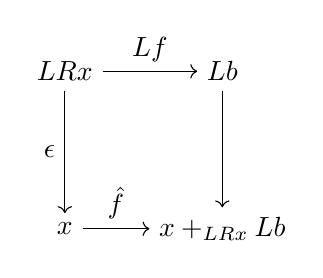
\begin{tikzpicture}
		\node (ul) at (0,2) {$ LRx $};
		\node (ll) at (0,0) {$ x $};
		\node (ur) at (2,2) {$ Lb $};
		\node (lr) at (2,0) {$ x +_{LRx} Lb$};
		\draw [->] (ul) to node [left] {$ \epsilon $} (ll);
		\draw [->] (ul) to node [above] {$ Lf $} (ur);
		\draw [->] (ll) to node [above] {$ \hat{f} $} (lr);
		\draw [->] (ur) to (lr);
	\end{tikzpicture}
	\] 
	Observe that $ R \hat{f} \from Rx \to R( x +_{LRx} Lb ) $. Also there is a string of isomorphisms  
	\[
		R( x +_{LRx} Lb ) \to Rx +_{RLRx} RLb \to Rx +_{Rx} b \to b
	\]
	whose composite we call $ h $. Then $ R \hat{f} = f . h^{-1} $ as desired.  \emph{(note: some details are needed here)}
	
	Now show that $ \hat{f} $ is cocartesian.  Consider a $ \D $-arrow $ g \from x \to y $ with a $ C $-arrow $ \theta \from R( x +_{LRx} Lb ) \to Ry  $ so that $ R \hat{f} . \theta = Rg $.  Can we uniquely lift $ \theta $? Set up the diagram
	\[
	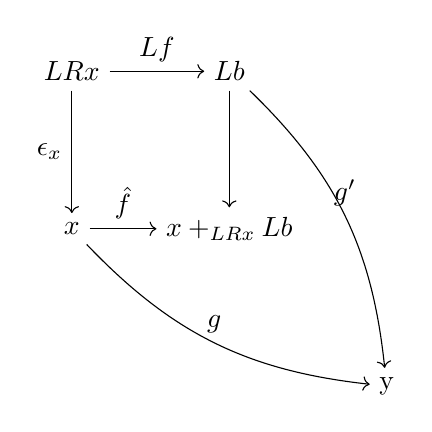
\begin{tikzpicture}
		\node (ul) at (0,2) {$ LRx $};
		\node (ll) at (0,0) {$ x $};
		\node (ur) at (2,2) {$ Lb $};
		\node (lr) at (2,0) {$ x +_{LRx} Lb$};
		\node (comp) at (4,-2) {y};
		\draw [->] (ul) to node [left] {$ \epsilon_x $} (ll);
		\draw [->] (ul) to node [above] {$ Lf $} (ur);
		\draw [->] (ll) to node [above] {$ \hat{f} $} (lr);
		\draw [->] (ur) to (lr);
		\draw [->] (ll) to [bend right=20] node [above] {$ g $} (comp);
		\draw [->] (ur) to [bend left=20] node [above] {$ g' $} (comp);
	\end{tikzpicture}
	\] 
	where $ g' \bydef Lh^{-1} . L\theta.\epsilon_y $.  To show the outer square commutes, it suffices to show that $ Lf . g' $ and $ \epsilon_x . g $ have the same image under the adjunction homset correspondence.  We have
	\[
		Lf . g' = Lf . Lh^{-1} . L\theta.\epsilon_y 
			\mapsto \eta_{Rx} . RLf . RLh^{-1} . RL\theta.R\epsilon_y 
			= f . h^{-1} . \theta  
			= R \hat{f} . \theta 
			= Rg
	\]
	and 
	\[
	\epsilon_x . g \mapsto \eta_{Rx} . Rg = Rg.	
	\]
\end{proof}

Perhaps it will be helpful to also tackle the special case of Grothendieck fibrations.

\begin{cnj}
If $\cat{C}$ and $\cat{D}$ have chosen pushouts (where a pushout of a morphism $f$ along the
identity `is' $f$) such that $R\colon\cat{D}\to\cat{C}$ strictly preserves them, then $R$ is an opfibration
when $R$ is a lari.
\end{cnj}

\begin{proof}
{\chris Wait for Lack's response to untangle the mess with chosen limits and colimits, and preserving them}
\end{proof}

For the converse, Gray already gives an answer for the Grothendieck case.

\begin{thm}
 {\chris write Gray and proof. Looks like choice issues are better understood here.}
\end{thm}

For the Street case, we can 'relax' the above, or go to a different direction as below. {(\chris write the relaxed Gray as well)}

\begin{thm}
	Given a Street opfibration $ R \from \cat{D} \to \cat{C} $, it is a right adjoint when it is \nice.
\end{thm}
 
Let's try to figure out what \nice could be. Here are some helpful theorems.

\begin{thm}[Freyd's general adjoint functor theorem]
\label{thm:GAFT}
	A functor $ F \from X \to Y $ is a right adjoint if  $ x $ is complete, locally small, and $ F $ satisfies the \emph{solution set condition}. The latter says, for any $ Y $-object $ y $, there exists a small set $ I $ indexing a collection of $ X $-objects $ {x_i}_I $ and $ Y $-arrows $ {f_i \from y \to F ( x_i ) } $ such that every $ F $-valued $ Y $-arrow $ y \to R x $ factors as $ Fg . f_k $ for $ k \in I $ and $ g \from x_k \to x $.
\end{thm}

\begin{proof}
	The proof is V.6.2 in CWM.  Define the left adjoint $ G \from Y \to X $ by $ G (y) \coloneqq x $ where $ y \to F x $ is initial in the comma category $ y \downarrow F $.  
\end{proof}

\begin{thm}[Gabriel-Zisman]
\label{thm:GabZis}
	An adjunction $ L \dashv R \from \cat{C} \leftrightarrow \cat{D} $. TFAE:
	\begin{enumerate}
		\item $ L $ is full and faithful;
		\item the unit is an isomorphism;
		\item the induced comonad on $ \cat{D} $ is idempotent, $ L $ is conservative, and $ R $ is essentially surjective.
	\end{enumerate}
\end{thm}

Now, let's prove a strong theorem then try to weaken it

\begin{thm}
	Let $ \cat{D}$ be locally small and complete. Also let $ R \from \cat{D} \to \cat{C} $ be a continuous, surjective-on-objects Grothendiek opfibration.  Then $ R $ is a right adjoint.
\end{thm}

\begin{proof}
	We use \ref{thm:GAFT}.  Suffice to show the solution set condition holds.  Fix a $ C $-objects $ c $.  Then the indexing set is $ \ast $, the collection of $ D $-objects consists of a single object $ x_c $ over $ c $ (which exists by surjective-on-objects assumption), and the collection of $ \cat{C} $-arrows consists of the identity.  Any map $ f \from c \to Rd $ has a cocartesian lifting $ \hat{f} \from x_c \to x_{Rd} $ and $ f = R \hat{f} . 1_c $.
\end{proof}

\begin{thm}
	Let $ \cat{D}$ be locally small and complete. Also let $ R \from \cat{D} \to \cat{C} $ be a continuous, surjective-on-objects, conservative Street opfibration.  Then $ R $ is a right adjoint.
\end{thm}

\begin{proof}
	We use \ref{thm:GAFT}.  Suffice to show the solution set condition holds.  Fix a $ C $-objects $ c $.  Then the indexing set is $ \ast $, the collection of $ D $-objects consists of a single object $ x_c $ over $ c $ (which exists by surjective-on-objects assumption), and the collection of $ \cat{C} $-arrows consists of the identity.  For any map $ f \from c \to Rd $, there exists an essential cocartesian lifting $ \hat{f} \from x_c \to d' $ together with a $ \cat{C} $-isomorphism $ h \from Rd' \to Rd $ such that $ f = h . R \hat{f} $. But $ f = h . R \hat{f} = R \hat{h} . R \hat{f} . 1_c = R (\hat{h} . \hat{f}) . 1_c $ where $ h = R \hat{h} $ because $ R $ is conservative.
\end{proof}

\begin{thm}
	Let $ \cat{D}$ be locally small and complete. Also let $ R \from \cat{D} \to \cat{C} $ be a continuous, essentially surjective, conservative Street opfibration.  Then $ R $ is a right adjoint.
\end{thm}

\begin{proof}
	We use \ref{thm:GAFT}.  Suffice to show the solution set condition holds.  Fix a $ C $-object $ c $.  Then the indexing set is $ \ast $, the collection of $ D $-objects consists of a single object $ d' $ where $ \theta \from c \cong Rd' $ (which exists by essential surjectivity), and the collection of $ \cat{C} $-arrows is $ { \theta } $.  For any $ \cat{C} $-arrow $ f \from c \to Rd $, we have (by Street opfibrationness) $ f . \theta^{-1} \from Rd' \to c \to Rd $, a cocartesian essential lifting $ \hat{ f . \theta^{-1} } \from d' \to d'' $ in $ \cat{D} $, and an isomorphism $ h \from d \to d'' $ (by conservatism) such that $ f . \theta^{-1} = Rh . R \hat{ f . \theta^{-1} } $.  This implies, as required by GAFT, that $ f = R (h\hat{ f . \theta }) . \theta $.
\end{proof}

Thoughts about these assumptions. Here are the desired examples I can think of now: $ \cat{Set} $ together with $ \cat{Graph} $ or $ \cat{Top} $. The enriched over sets and completeness are both there. So is essential surjectivity. And reflection of isomorphisms.  The continuity is definitely needed, since it's necessary if $ R $ is a right adjoint. 

Go back to the right adjoint we had in the ``converse'' to the above theorem.  That is, we have a coreflection $ L \dashv R \from \cat{C} \leftrightarrow \cat{D} $ where $ L $ is left exact.  Of course this gives the continuity of $ R $. Essential surjectivity follows from Gabriel-Zisman. Is it a Street opfibration? $ L $ is conservative, but is $ R $?

\begin{ex}
	No, $ R $ is not in general conservative.  Consider the underlying node functor $ \Graph \to \Set $.  All $ \Graph $-endomorphisms on
	\[
	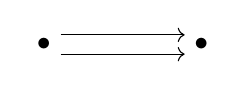
\begin{tikzpicture}
		\node (a) at (0,0) {$ \bullet $};
		\node (b) at (2,0) {$ \bullet $};
		\draw [->] (a.30) to (b.150);
		\draw [->] (a.-30) to (b.-150);
	\end{tikzpicture}
	\]
	are sent to the identity on $ 2 $.
\end{ex}

At this point, we have partial converses:

\fbox{
\begin{minipage}{0.4\textwidth}
		Let $ \D $ have pushouts. Given a coreflection $ L \dashv R \from \C \to \D $ where $ R $ preserves pushouts, $ R $ is a Street opfibration.
\end{minipage}
}
\hfill
\fbox{
\begin{minipage}{0.4\textwidth}
		Let $ \cat{D}$ be locally small and complete. Also let $ R \from \cat{D} \to \cat{C} $ be a continuous, essentially surjective, conservative Street opfibration.  Then $ R $ is a right adjoint.
\end{minipage}
}


\bibliographystyle{alpha}
\bibliography{references}



\end{document}

